\documentclass[11pt]{article}
\usepackage{Sweave}
\begin{document}
\section{Introduction}
Let's first simulate some data.
\begin{Schunk}
\begin{Sinput}
> x <- rnorm(100)
> y <- x + rnorm(100, sd = 0.5)
\end{Sinput}
\end{Schunk}
Here is a scatterplot of the data.
\begin{Schunk}
\begin{Sinput}
> par(mar = c(5, 4, 1, 1), las = 1)
> plot(x, y, main = "My Data")
\end{Sinput}
\end{Schunk}
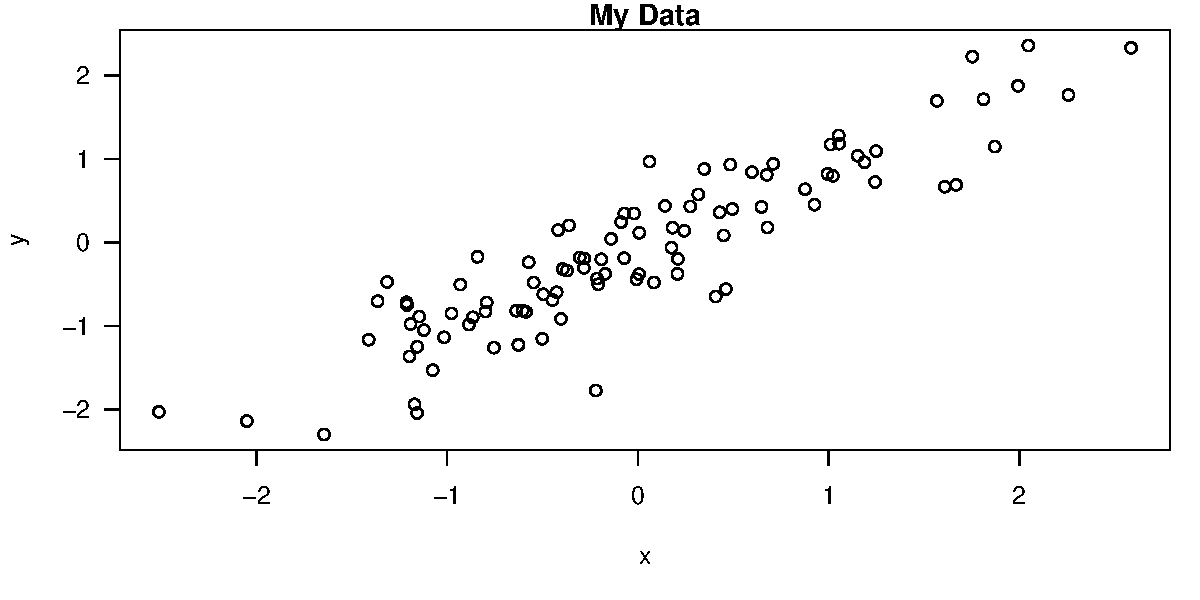
\includegraphics{example5-scatterplot}
\end{document}
